% SPDX-License-Identifier: CC-BY-SA-4.0
% SPDX-FileCopyrightText: Louis Royer <infos.louis.royer@gmail.com>
\documentclass[../main.tex]{subfiles}
\begin{document}
\initSubfile[1]
\chapter{Aperçu des réseaux mobiles de 5\textsuperscript{ème} génération et de l'\textit{edge computing}}
\label{ch:overview-5G-edge}
\begin{chapterHeader}
Ce chapitre a pour objectif de présenter les fondements techniques et conceptuels nécessaires à la compréhension des réseaux mobiles de 5\textsuperscript{ème} génération (5G) et de l’\textit{edge computing}, ainsi que les enjeux liés à leur intégration. Il re-trace d’abord les évolutions architecturales et fonctionnelles des réseaux mobiles au cours des générations, en mettant en évidence les ruptures technologiques qui ouvrent la voie à de nouveaux usages. Il expose ensuite les principes de l’\textit{edge computing} comme modèle complémentaire au \textit{cloud computing}, en soulignant son rôle central dans le traitement distribué de données et l’optimisation des performances.
\end{chapterHeader}

\section{Réseaux mobiles de 5\textsuperscript{ème} génération}
La connectivité à Internet est devenue essentielle à la vie quotidienne des citoyens.
Avec la démocratisation des \textit{smartphones} couplée au déploiement de la technologie \acren{LTE}, les réseaux mobiles sont devenus incontournables.

Face à l’augmentation du nombre d’appareils connectés et des volumes de données échangées, la technologie radio de la 4G montre ses limites~\cite{10.1007/s11276-020-02479-w,10.1016/j.array.2022.100170}. Le \acren{3GPP} s’appuie donc sur des technologies de rupture afin de combler les lacunes de la 4G en standardisant la 5G dans sa \textit{release}~15 et les \textit{releases} suivantes.

Les premières évolutions visibles par les utilisateurs finals concernent le changement de technologie radio. Le passage à la technologie \acren{5G NR} nécessite des \acrfrpl{UE} compatibles à la fois avec les porteuses radio et avec les protocoles de la 5G. Il s’agit du déploiement de la 5G \acren{NSA} qui conserve le \gl{ePC}{cœur de réseau 4G (\textit{evolved~Packet~Core},~ePC)} existant et se concentre sur l’évolution du \acren{RAN}.

Mais pour déployer de la 5G \acren{SA}, les opérateurs doivent remplacer leur ePC par un \gl{5GC}{cœur 5G (\textit{5G Core}, 5GC)}. Ils peuvent alors bénéficier de toutes les fonctionnalités de la 5G, supposées servir de fondation au développement de nouvelles applications comme l’\acrfr{IIoT}, les \acrfr{CITS}, la santé connectée (\textit{eHealth}) ou encore la \acrfr{XR}.

\begin{figure}[h]
    \centering
    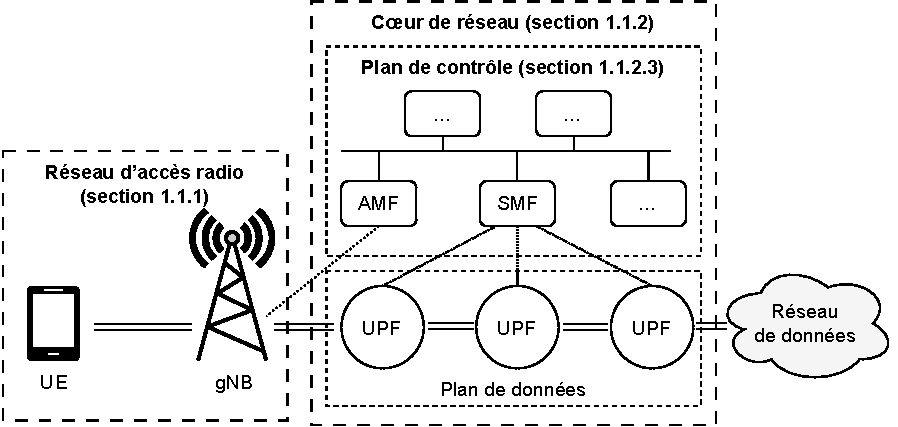
\includegraphics[width=0.77\linewidth]{figs/presentation-5G.drawio.pdf}
    \caption[Architecture~5G simplifiée]{Architecture 5G simplifiée}
    \label{fig:architecture-5G-simplifiée}
\end{figure}

Nous présenterons en premier lieu l’architecture de la 5G, dont la figure~\ref{fig:architecture-5G-simplifiée} est une représentation simplifiée.
Nous commencerons par un bref tour d’horizon des nouveautés relatives à l’accès radio (section~\ref{sec:RAN}), qui même s’il est l’un des aspects les plus remarqués par les utilisateurs ne constitue pas le cœur de cette thèse. Puis nous adopterons une approche chronologique pour présenter le cœur de réseau (section~\ref{sec:CN}).
Et enfin, nous présenterons quelques notions essentielles avant de donner un aperçu de l’évolution en cours vers la 6\textsuperscript{ème} génération.

\pagebreak

\subsection{Accès radio}
\label{sec:RAN}
\subsubsection{Débits}
La technologie \gl{5G NR}{\textit{New Radio} (NR)} intègre les dernières avancées scientifiques et technologiques, ce qui permet à la 5G de fournir des débits considérablement plus élevés que la 4G~\cite{10.1016/j.comnet.2024.110370}. Le \acren{MIMO}, le \textit{beamforming}, \acrfr{DSS}, la \textit{Dual Connectivity} et l’agrégation de porteuses (\textit{Carrier Aggregation}) permettent de réduire les interférences et d’obtenir une latence faible~\cite{10.1109/WPMC50192.2020.9309496}.
L’utilisation conjointe des bandes Sub-6~GHz et des bandes millimétriques se traduit en une augmentation des débits. Pour les communications descendantes, il est possible d’agréger jusqu’à 8 \textit{layers}, et 4 pour les communications montantes ; dans le tableau~\ref{table:debits5GNR}, les débits sont donc à multiplier par 8 et par 4 respectivement pour obtenir les débits maximums par porteuse. 

\begin{table}[h]
\centering
\scalebox{0.9}{
\begin{tabular}{lcccc}
\toprule
\thead{Bande de\\ fréquences} & \thead{Espacement des\\ sous-porteuses\\ (kHz)} & \thead{Bande passante\\ (MHz)} & \thead{Débit descendant\\ (Mb/s)} & \thead{Débit montant\\ (Mb/s)} \\
\midrule
FR1                         & 15                                           & 50                            & 361                              & 309                           \\
FR1                         & 30                                           & 100                           & 730                              & 625                           \\
FR1                         & 60                                           & 100                           & 722                              & 618                           \\
FR2-1                       & 60                                           & 200                           & 1078                             & 887                           \\
FR2-1                       & 120                                          & 400                           & 2155                             & 1774                          \\
FR2-2                       & 480                                          & 1600                          & 8097                             & 6665                          \\
FR2-2                       & 960                                          & 2000                          & 9664                             & 7955                         \\
\bottomrule
\end{tabular}
}
\caption[Débits théoriques de la 5G]{Débits maximums par \textit{layer} par bande agrégée~\cite{10.1007/978-3-031-82830-0_8}}.
\label{table:debits5GNR}
\end{table}

\subsubsection{Séparation de la station de base entre CU et DU}
\label{sec:CU/DU}

\begin{wrapfigure}{r}{0.45\textwidth}
    \centering
    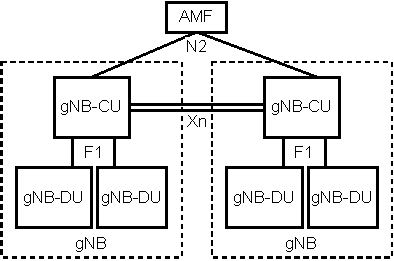
\includegraphics[width=0.85\linewidth]{figs/RAN-CU-DU.drawio.pdf}
    \caption[Séparation de la station de base entre unité centralisée et unités distribuées]{\gl{CU/DU}{Séparation de la gNB en} \protect\linebreak \gl{CU/DU}{CU (\textit{Central Unit}) et DU (\textit{Distributed Unit})}~\cite{3GPP.TS.38.401}.}
    \label{fig:RAN-CU-DU}
\end{wrapfigure}

En 5G, l’architecture des stations de base est repensée pour offrir plus de modularité: la \gl{gNB}{gNB (\textit{Next Generation Node B})} \gl{CU/DU}{sépare ses fonctionnalités entre une unité centralisée (\textit{Central Unit}, CU) et des unités distribuées (\textit{Distributed Units}, DUs)}, comme illustré par la figure~\ref{fig:RAN-CU-DU}.

Les \gl{DU}{unités distribuées} sont physiquement présentes au plus proche des \gl{RU}{unités radio (\textit{Radio Units}, RUs)} afin de limiter les pertes, alors que les \gl{CU}{unités centralisées} peuvent être virtualisées dans des \gl{datacenter}{centres de données}.

Cette modularité établit les bases pour la définition de l’architecture \acrfr{O-RAN}, qui permet notamment d’intégrer le \gl{slice}{\textit{network slicing}} dans le \acren{RAN}, d’améliorer la gestion de la mobilité et d’optimiser la consommation d’énergie du \acren{RAN}~\cite{10.1109/OJCOMS.2024.3430823} et l’émergence de son écosystème ouvert et interopérable.

\subsection{Architecture du cœur de réseau 5G}
\label{sec:CN}
\subsubsection{Cœur de réseau « tout IP» de la 4G}
En 2008, le \acren{3GPP} standardise la 4G dans sa 8\textsuperscript{ème}~\textit{release}~\cite{3GPP.TS.23.401}.
Cette génération utilise désormais un \acrfr{CN} « tout IP »: l’\acren{ePC}. Comme illustré sur la figure~\ref{fig:4G-EPC}, il est composé initialement de 5~entités:

\begin{itemize}
    \item la \acren{MME} qui est responsable de la signalisation avec l’\acren{E-UTRAN};
    \item le \acren{HSS} pour stocker les données relatives aux \acrfrpl{user};
    \item la \acren{SGW} responsable de l’interconnexion avec l’\acren{E-UTRAN};
    \item la \acren{PGW} responsable de l’interconnexion avec le \acrfr{DN};
    \item la \acren{PCRF} pour gérer la politique de \acrfr{QoS} et la facturation.
\end{itemize}

\begin{figure}[h]
    \centering
    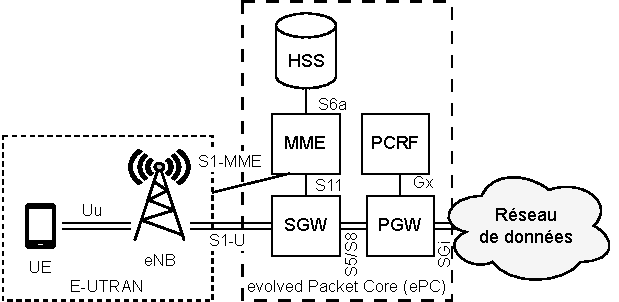
\includegraphics[width=0.9\linewidth]{figs/4G-EPC.drawio.pdf}
    \caption[Architecture d’un système 4G \textit{release}~8]{Architecture simplifiée d’un système 4G \textit{release}~8~\cite{3GPP.TS.23.401}}.
    \label{fig:4G-EPC}
\end{figure}

Dans cette \textit{release}, la \acren{SGW} et la \acren{PGW} gèrent à la fois le plan de contrôle et le plan utilisateur.

Avec sa \textit{release}~11, le \acren{3GPP} ajoute ensuite la \acren{TDF}, qui permet d’analyser le trafic pour classifier les différents flux de données selon le type d’application et ainsi faciliter la mise en œuvre de la politique de \acrfr{QoS}~\cite{10.1109/ICC.2012.6364750,3GPP.TS.23.203}.
\pagebreak

\subsubsection{Séparation du plan de contrôle et du plan utilisateur}
\label{sec:CUPS}
Pour faire face à l’augmentation du trafic, les opérateurs doivent ajouter régulièrement des équipements sur le réseau.
Pour réduire les coûts, il devient alors nécessaire de pouvoir faire évoluer \gl{CUPS}{séparément plan de contrôle indépendant du plan utilisateur}~\cite{3GPP.NEWS.2017.CUPS}.
C’est pourquoi le \acren{3GPP} crée l’\gl{CUPS}{architecture CUPS (\textit{Control and User Plane Separation})} dans sa \textit{release}~14~\cite{3GPP.TS.23.214}: la \acren{SGW}, la \acren{PGW} et le \acren{TDF} sont divisés chacun entre une entité centralisée responsable du contrôle et des entités distribuées chargées du traitement des paquets du plan utilisateur.
Plusieurs fonctions du plan utilisateur peuvent se partager une même fonction du plan de contrôle, ce qui permet de centraliser la gestion du réseau.

\begin{figure}[h]
    \centering
    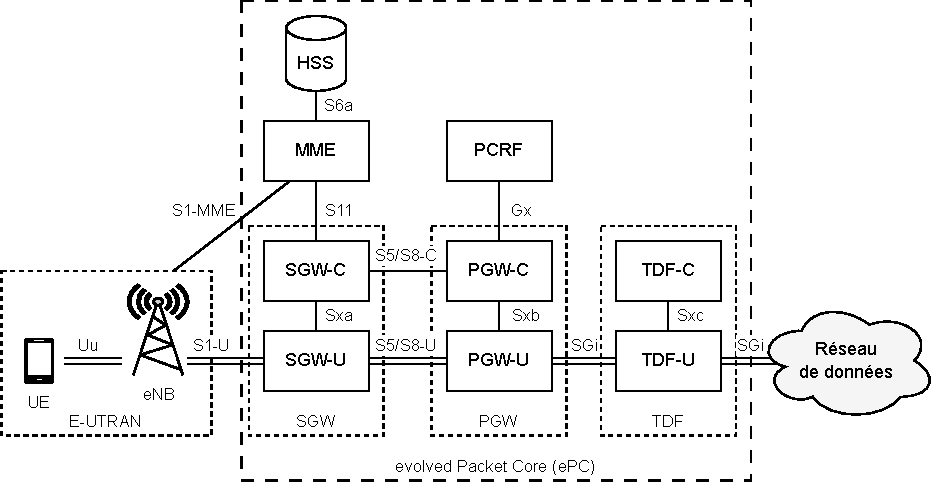
\includegraphics[width=0.95\linewidth]{figs/4G_CUPS.drawio.pdf}
    \caption[Architecture d’un système 4G \textit{release}~14]{Architecture d’un système 4G \textit{release}~14~\cite{3GPP.TS.23.214}.}
    \label{fig:4G-CUPS}
\end{figure}

Le protocole \acren{PFCP} permet l’injection de règles de traitement en utilisant les interfaces « Sx », comme illustré sur la figure~\ref{fig:4G-CUPS}. Cette nouvelle architecture utilise ainsi une partie du paradigme \acren{SDN}~\cite{10.1002/9781119629658.ch1}.

\subsubsection{Architecture basée sur des services}
\label{sec:SBA}
Cependant, malgré cette séparation, il subsiste certaines redondances entre les différentes fonctionnalités de ces entités.
Il est donc nécessaire de faire évoluer encore l’architecture pour mieux les répartir.

En outre, pour permettre une répartition optimale, il devient indispensable de découpler le matériel physique des couches logicielles.
Ce découplage doit rendre possible l’utilisation de matériel générique dans des \gl{datacenter}{centres de données} existants plutôt que de déployer un réseau dédié.

\pagebreak
En s’appuyant sur la \acrfr{NFV}, la 5G gagne en flexibilité et facilite le \gl{scalability}{passage à l’échelle}: l’\gl{SBA}{architecture est désormais basée sur des services (\textit{Service Based Architecture}, SBA)}, comme illustré sur la figure~\ref{fig:5G-system}. Ces services prennent la forme de \acrfrpl{NF} qui exposent des \gl{API}{APIs} \gl{REST}{REST}. 

\begin{figure}[h]
    \centering
    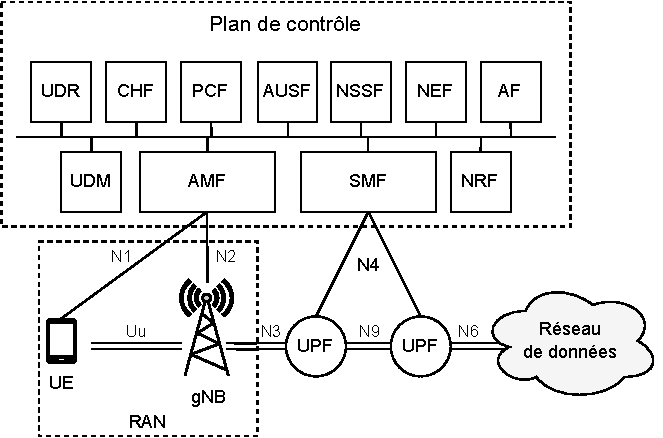
\includegraphics[width=0.75\linewidth]{figs/5GSystem.drawio.pdf}
    \caption[Architecture d’un système 5G]{Architecture de la 5G~\cite{3GPP.TS.23.501}.}
    \label{fig:5G-system}
\end{figure}

La 5G vient donc séparer les fonctions de gestion des sessions, de gestion de l’accès et de la mobilité, et d’authentification entre trois nouvelles fonctions qui viennent remplacer la \acren{MME}: la \acren{SMF}, l’\acren{AMF} et l’\acren{AUSF}.

Toutes les entités du plan utilisateur sont regroupées en une seule fonction: l’\acren{UPF}.
Cette fonction est à la fois capable d’effectuer le routage des paquets tout en appliquant la politique de qualité de service, et d’effectuer des relevés de consommation de données.

La \acren{PCRF} est remplacée par la \acren{PCF} et la \acren{CHF}, et la \acren{HSS} est remplacée par deux fonctions: l’\acren{UDR} et l’\acren{UDM}.

De nouvelles \acrenpl{NF} sont également définies pour proposer de nouvelles fonctionnalités ; par exemple:
\begin{itemize}
   \item le \acren{NRF} sert d’annuaire des \acrenpl{NF};
   \item la \acren{NSSF} permet de gérer les \acrenpl{slice} (voir section~\ref{sec:slice});
   \item la \acren{NEF} permet d’interface le \gl{5GC}{cœur 5G} avec des fonctions tierces (les \gl{AF}{\textit{Application Functions}, AFs}).
\end{itemize}

\pagebreak
\subsubsection{Notion de session PDU}
\label{sec:pdu-session}
En 5G, le type de données transportées n’est pas restreint aux paquets~IP: il est prévu par le standard de pouvoir utiliser d’autres types de données, comme des trames ethernet ou autres structures non spécifiées (\textit{unstructured}). C’est pourquoi en 5G on parle désormais de « \gl{PDU}{PDUs} », notion plus large que celle de « paquets ».

\begin{figure}[h]
    \centering
    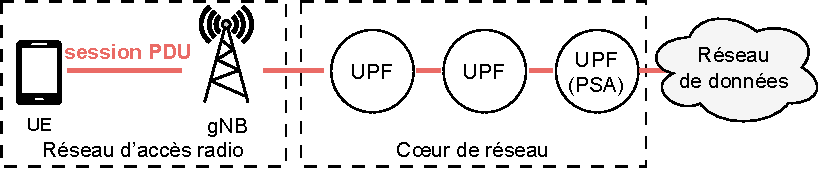
\includegraphics[width=0.67\linewidth]{figs/PDU-Session.drawio.pdf}
    \caption[Session PDU]{Une \gl{PDU Session}{session PDU} fournit une connectivité de bout-en-bout entre un \gl{UE}{équipement utilisateur} et un \gl{DN}{réseau de données}.}
    \label{fig:pdu-session}
\end{figure}

Une \acrfr{PDU Session} fournit une connectivité de bout-en-bout entre un \acrfr{UE} et un \gl{DN}{réseau de données}.
Pour établir cette connectivité, il est nécessaire d’établir un chemin sur \gl{CUPS}{plan utilisateur}, constitué de plusieurs \acrenpl{UPF} ; on appelle \acren{PSA} le dernier UPF de ce chemin, qui fait l’interconnexion avec le \gl{DN}{réseau de données}, comme illustré sur la figure~\ref{fig:pdu-session}.

\subsubsection{Gestion de la mobilité}
\label{sec:mobility}
Lorsqu’un utilisateur se déplace, il est nécessaire de changer de station de base: ce changement est appelé un \gl{handover}{\textit{handover}}. On désigne par « \acren{gNB} source » la \acren{gNB} qui était utilisée par l’utilisateur au début de ce processus, et par « \acren{gNB} cible » celle qui est utilisée à la fin.

Tout l’enjeu du \gl{handover}{\textit{handover}} est de changer le point d’entrée dans le réseau 5G pour un \acrfr{UE} de manière transparente pour l’utilisateur: ses applications doivent pouvoir continuer de fonctionner sans interruption. Pour permettre cette continuité de service, il est nécessaire pour la \acren{gNB} source de transférer vers la gNB cible les \acrenpl{PDU} à destination de l’\acrfr{UE} qui lui parviendront après le départ de celui-ci: on appelle cette opération le \textit{forwarding}.

Le \gl{handover}{\textit{handover}} se déroule en deux phases: d’abord une phase de préparation qui sert à re-configurer les équipements du \acrfr{CN} avant que le changement de \acren{gNB} soit effectif, puis une phase d’exécution qui vient valider le \gl{handover}{\textit{handover}}.

Il existe en 5G plusieurs types de \gl{handover}{\textit{handover}}:
\begin{itemize}
    \item Le \gl{handover}{\textit{handover}}~Xn peut être utilisé s’il existe un lien radio entre les \acrenpl{gNB} source et cible (interface~Xn): ce type de \gl{handover}{\textit{handover}} est initié par les \acrenpl{gNB} sur la base de mesures périodiques de qualité de signal. Il ne permet pas le changement d’AMF, et le \textit{forwarding} se fait de manière directe en utilisant l’interface~Xn.
    \item Le \gl{handover}{\textit{handover}}~N2 peut être utilisé dans les autres cas de figure: ce type de \gl{handover}{\textit{handover}} peut être initié soit par la \acren{gNB} soit par l’\acren{AMF}. Il permet le changement d’AMF, et le \textit{forwarding} se fait en utilisant le protocole \gl{GTP}{GTP}, soit de manière directe entre les deux \acrenpl{gNB}, soit de manière indirecte en passant par un \acren{UPF}.
\end{itemize}
\pagebreak

Une fois le \gl{handover}{\textit{handover}} effectué, il est possible que l’\acren{UPF} servant de \acren{PSA} qui avait été sélectionné lors de l’établissement de la \acrfr{PDU Session} soit placé de manière sous-optimale, et il est alors nécessaire d’en sélectionner un autre. Lorsque le \acrfr{DN} est un réseau IP, ce changement implique un changement d’adresse IP pour l’\acrfr{UE}.

\begin{figure}[h]
    \centering
    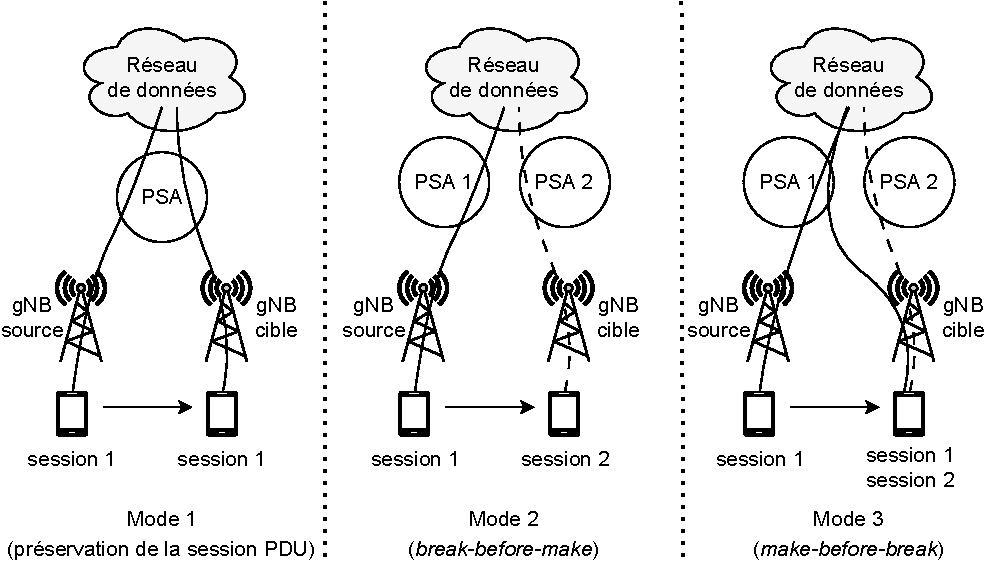
\includegraphics[width=1\linewidth]{figs/SSC-modes.drawio.pdf}
    \caption[Modes de continuité de service et de session]{Il existe 3~modes de continuité de service et de session.}
    \label{fig:ssc-modes}
\end{figure}

Selon l’application, ce changement peut avoir un impact négatif sur l’\gl{QoE}{expérience utilisateur}. Les~3~modes de gestion de la \gl{SSC}{continuité de service et de session (\textit{Service and Session Continuity}, SSC}) sont résumés sur la figure~\ref{fig:ssc-modes}:

\begin{itemize}
    \item le premier consiste à conserver le même \acren{PSA} pendant toute la durée de vie de la \acrfr{PDU Session};
    \item le deuxième consiste à interrompre la \acrfr{PDU Session} puis en créer une nouvelle (\textit{break-before-make});
    \item et le troisième à créer une nouvelle \acrfr{PDU Session} puis supprimer l’ancienne (\textit{make-before-break}).
\end{itemize}

Lorsqu’une application est capable de gérer deux \acrfrpl{PDU Session} simultanément, utiliser le dernier mode permet d’obtenir la qualité de service optimale sans interruption de service.
Dans le cas contraire, si l’application tolère la perte de connectivité temporaire il est possible d’utiliser le deuxième mode.
Le premier mode sera utilisé par défaut dans les autres situations: il ne permet pas de modifier le \acren{PSA}.

\pagebreak
\subsubsection{Notion de \textit{slice}}
\label{sec:slice}
Pour permettre de fournir des services adaptés à chaque application, la 5G intègre dans sa conception la notion de \acrenpl{slice}.

Une \gl{slice}{\textit{slice}} est une partition du réseau constituée d’un ensemble de ressources disponibles au sein d’une infrastructure mutualisée. Chaque \gl{slice}{\textit{slice}} est isolée et gérée indépendamment des autres, et est dédiée à un type de service spécifique.

Le standard~5G définit initialement trois types de \acrenpl{slice}: \acren{eMBB}, \acren{URLLC} et \acren{MIoT}, puis ajoute dans les quatre \textit{releases} successives les types de \acrenpl{slice} \acren{V2X}, \acren{HMTC}, \acren{HDLLC}, et \acren{GBRSS}~\cite{3GPP.TS.23.501}.

\begin{figure}[h]
    \centering
    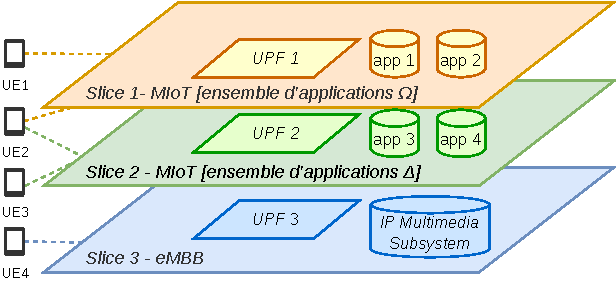
\includegraphics[width=0.8\linewidth]{figs/slicing.drawio.pdf}
    \caption[Notion de \textit{slice}]{Un réseau mobile peut proposer plusieurs \acrenpl{slice} à ses utilisateurs. Chaque \gl{PDU Session}{session PDU} d’un équipement utilisateur est associé à une \acren{slice} parmi celles qui lui sont autorisées par l’opérateur, et peut utiliser uniquement les ressources disponibles pour cette \acren{slice}.}
    \label{fig:slicing}
\end{figure}

Les opérateurs n’implémentent pas nécessairement tous les types de \acrenpl{slice} au sein de leur réseau. Par exemple sur la figure~\ref{fig:slicing}, l’opérateur implémente une \acren{slice} de type \acren{eMBB} et deux \acrenpl{slice} de type \acren{MIoT} proposant chacune un ensemble de ressources et d’application différentes.

\subsection{Vers la 6G}
% fait office de mini-conclusion
La \textit{release}~20 du standard \acren{3GPP} étudiera les exigences pour la~6G selon les usages envisagés, mais elle ne sera publiée dans sa version finale qu’en mars 2027. Le travail normatif aura lieu avec la \textit{release}~21 dont l’échéancier sera défini au plus tard en juin~2026~\cite{3GPP.NEWS.2025.REL20.PLANNING}.

Les versions préliminaires des études de la \textit{release}~20 sont des documents internes au \acren{3GPP}, et il n’est donc pas possible de connaître le contenu de ces documents. Néanmoins, nous pouvons nous fonder sur le résumé du \textit{workshop}~6G du \acren{3GPP}~\cite{3GPP.WS.2025.6G.SUMMARY} pour connaître les domaines d’intérêt des membres du \acren{3GPP} et profiler les tendances.

\subsubsection{Simplification et optimisations de l’architecture}
Le mécanisme de transition de la~5G (\acren{NSA} puis \acren{SA}) s’est avéré complexe et difficile à mettre en œuvre pour les opérateurs; il est envisagé de proposer en priorité un mode \acren{SA} pour la~6G et d’éviter les options \acren{NSA} dans la mesure du possible afin de faciliter les déploiements. Dans la même optique, le nombre de configurations possibles de l’architecture des systèmes~6G sera réduit et les \acrenpl{NF} seront davantage découplées pour éviter les fonctionnalités redondantes. Le \gl{CN}{cœur de réseau} utilisera des versions plus modernes des protocoles.

Ces changements s’inscrivent dans la continuité des changements apportés par les générations précédentes, et il est clair que le \acren{3GPP} veut se concentrer sur une propriété importante mais difficile à obtenir: la simplicité.

\subsubsection{Connectivité ubiquitaire avec l’intégration aux réseaux non-terrestres}
Les travaux d’intégration des \gl{NTN}{réseaux non-terrestres (NTN)} avaient déjà commencé avec les \textit{releases}~17 et 18, et les membres du \acren{3GPP} ont montré un intérêt clair pour les poursuivre afin d’unifier les architectures des réseaux terrestres et \gl{NTN}{non-terrestres}. Cette unification vise à obtenir dès le premier jour du déploiement une meilleure couverture radio pour la 6G que pour la 5G, mais nécessitera des changements d’interface radio qui rendront probablement les équipements non rétro-compatibles.

Nous pouvons prévoir que l’\textit{edge computing} aura une place importante dans ce modèle, car il est indispensable pour espérer obtenir une bonne \gl{QoE}{expérience utilisateur} malgré les contraintes de latence et de débit des liens satellitaires.  

\subsubsection{Intégration avec les technologies d’intelligence artificielle}
Le \acren{3GPP} souhaite faciliter l’intégration des technologies d’intelligence artificielle/d’apprentissage machine (\textit{Artificial Intelligence}/\textit{Machine Learning}, AI/ML) au sein de la 6G~\cite{3GPP.NEWS.2025.AIML}. Le \acren{3GPP} ne standardisera \textit{a priori} pas les modèles d’AI/ML en eux-même: son travail s’oriente vers la création de mécanismes qui permettent l’utilisation de modèles existants.

Parmi les multiples cas d’usages, on retrouve notamment les « jumeaux numériques » (\textit{digital twin}): il s’agit de localiser en temps réel des éléments dans un environnement en 3~dimensions afin de les représenter dans un environnement numérique. Cette technologie permet de superviser un environnement réel, de simuler des actions sur sa représentation numérique, voire même d’effectuer à distance des opérations réelles (télémédecine, conduite de véhicules, \textit{handover} intelligent, etc.)~\cite{10.1109/MCOM.001.21143}.

Ces traitements ont des contraintes temporelles fortes lorsqu’il y a interaction avec l’environnement physique, et une fois encore l’\textit{edge computing} semble indispensable à cette intégration.

\pagebreak
\section{\textit{Edge computing}}
\label{sec:edge-computing}
Aujourd'hui, le \textit{cloud computing} est le modèle prédominant pour déployer des services sur Internet. Il permet de réduire les coûts de déploiement des applications en mutualisant les ressources d’hébergement tout en conservant suffisamment de flexibilité pour permettre de proposer les services à un grand nombre d’utilisateurs~\cite{10.1109/CloudSummit47114.2019.00007}.

Dans ce modèle, les données sont traitées de manière centralisée dans un nombre limité de \gl{datacenter}{centres de données}. Plus l’utilisateur final est éloigné du \gl{datacenter}{centre de données}, plus la nature centralisée du \textit{cloud computing} montre ses limites: les performances de la communication se dégradent avec la distance.
Pour atténuer les effets de la distance, des \acrenpl{CDN} sont déployés sur l’ensemble du globe: l’objectif est de mettre en cache les contenus les plus populaires, afin de pouvoir le transmettre plus rapidement aux utilisateurs qu’en contactant le \gl{datacenter}{centre de données}, comme illustré sur la figure~\ref{fig:cdn-cloud}.

\begin{figure}[h]
    \centering
    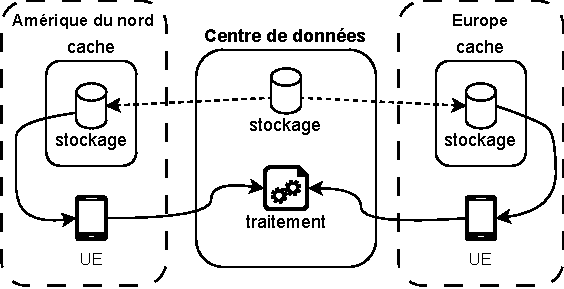
\includegraphics[width=0.6\linewidth]{figs/cdn-cloud.drawio.pdf}
    \caption[Modèle du \textit{cloud computing}]{Dans le modèle du \textit{cloud computing} les ressources de calcul ne sont disponibles que dans le \gl{datacenter}{centre de données}. Seul le stockage peut être distribué au sein du réseau.}
    \label{fig:cdn-cloud}
\end{figure}

Mais pour les applications où un traitement en temps réel des données des utilisateurs est nécessaire, les \acrenpl{CDN} ne répondent pas au besoin: ils permettent uniquement le stockage de données. Pour permettre à ces applications de fonctionner, il est donc nécessaire de changer de modèle et de distribuer sur le réseau non seulement le stockage mais également les ressources de calcul. 

L’\textit{edge computing} est une évolution du modèle de \textit{cloud computing} qui vient répondre à ce problème~\cite{10.1016/j.future.2019.02.050}. Il permet d’effectuer les traitements de données en périphérie du réseau, c’est-à-dire au plus proche de la source des données. Cette particularité fait de l’\textit{edge computing} le modèle idéal pour les équipements limités en ressources (\gl{IoT}{Internet des objets}, systèmes embarqués, etc.) qui peuvent ainsi à la fois prolonger leur durée de fonctionnement en se délestant sur le réseau des tâches les plus coûteuses en énergie, mais également effectuer rapidement des calculs qui n’étaient pas envisageables auparavant faute de ressources suffisantes.

\subsection{Architecture MEC de l’ETSI}
\label{sec:MEC}
Dès septembre~2014, l’\gl{ETSI}{ETSI} forme un Groupe de Spécification pour l’Industrie (\textit{Industry Specification Group}, ISG) dédié au \gl{MEC}{\textit{Mobile Edge Computing} (MEC)}~\cite{ETSI.GR.MEC.WP.1,ETSI.GR.MEC.HOMEPAGE}.
Cet ISG standardise l’architecture MEC~\cite{ETSI.GS.MEC.003}. En 2018, le périmètre de l’ISG s’élargit pour permettre une convergence entre réseaux mobiles, réseaux fixes~\cite{ETSI.GS.MEC.029}, et Wi-Fi~\cite{ETSI.GS.MEC.028}; l’architecture est donc renommée en \textit{Multi-access Edge Computing} en conservant l’acronyme « MEC ». Cette architecture permet de fédérer plusieurs systèmes \acren{MEC} au travers d’\acrenpl{API} standardisées.

L’architecture MEC de l’ETSI est un environnement \textit{Edge Native}~\cite{ETSI.GR.MEC.WP.55}, c’est-à-dire que les applications qui y sont déployées sont conçues pour exploiter les caractéristiques de l’\textit{edge computing}: ces applications prennent la forme de micro-services dans des conteneurs et doivent être en mesure de s’intégrer avec les différentes \acrenpl{API} proposées par cette architecture.

\subsubsection{Vue d’ensemble}
Le \textit{framework}~MEC (voir figure~\ref{fig:etsi-mec-framework}) est composée de 3~couches~\cite{IEEE.5G.Tech.Focus.2017}: 
\begin{itemize}
    \item La couche « système MEC » est chargée principalement de l’orchestration des ressources de l’ensemble du système.
    \item La couche « hôte MEC » est formée par l’ensemble des hôtes MEC ainsi qu’un système de gestion de cette couche.
    \item La couche « réseaux » permet la connectivité avec les réseaux de données.
\end{itemize}

\begin{figure}[h]
    \centering
    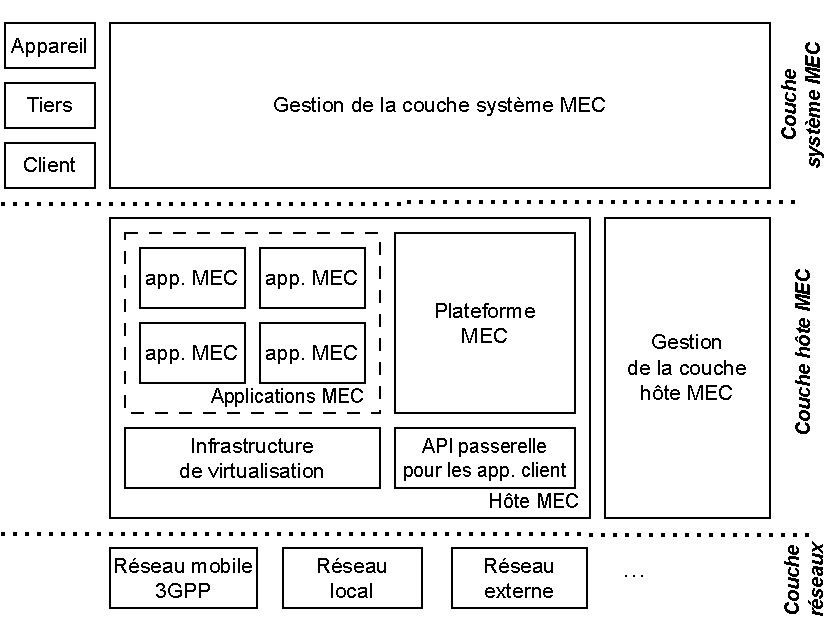
\includegraphics[width=0.7\linewidth]{figs/ETSI_MEC_framework.drawio.pdf}
    \caption[Vue d’ensemble du \textit{framework} \textit{Multi-Access Edge Computing} de l’ETSI]{Vue d’ensemble du \textit{framework} \textit{Multi-Access Edge Computing} de l’ETSI~\cite{ETSI.GS.MEC.003}.}
    \label{fig:etsi-mec-framework}
\end{figure}

L’architecture de référence, illustrée par la figure~\ref{fig:etsi-architecture-mec}, n’inclut que les deux premières couches puisque cette architecture se veut agnostique de la technologie utilisée pour le réseau de données.

 
\begin{figure}[h]
    \centering
    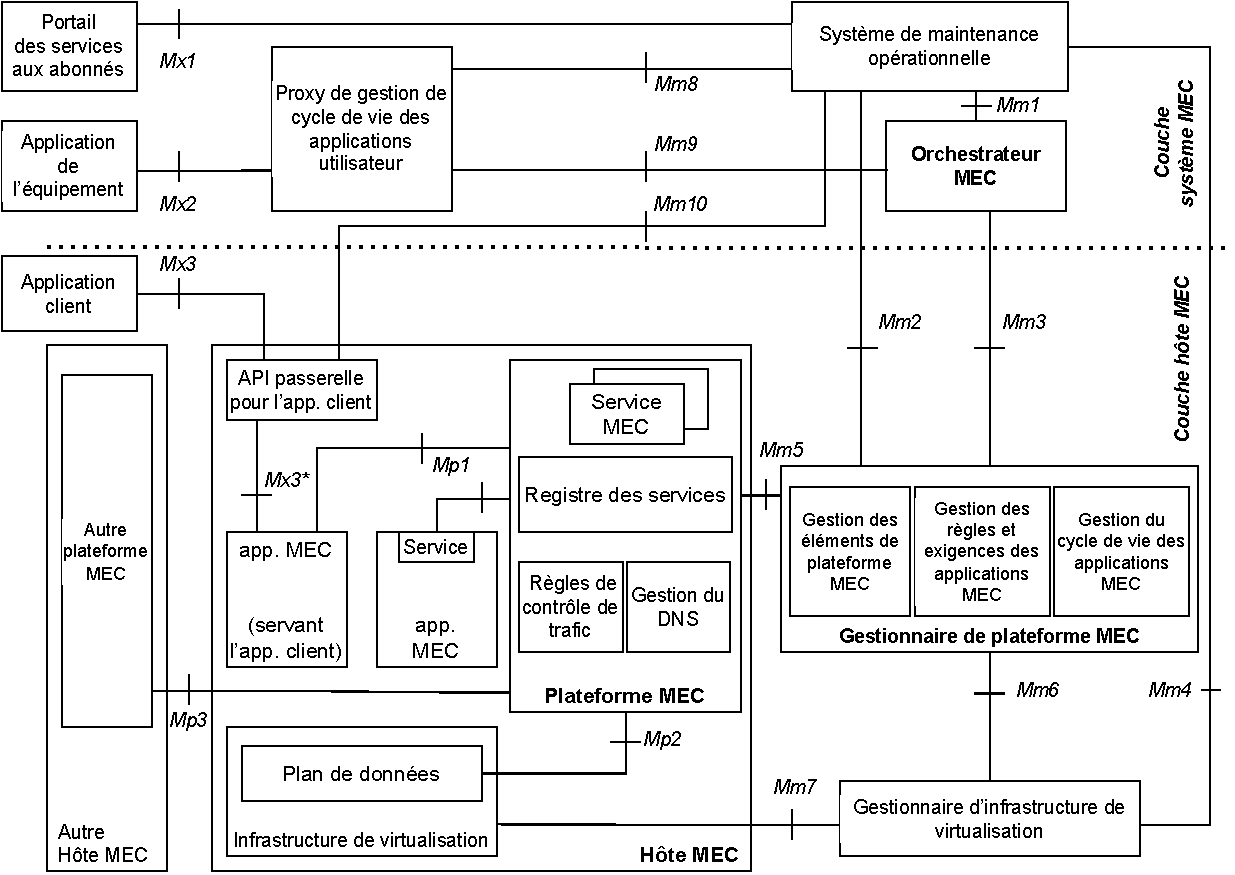
\includegraphics[width=1\linewidth]{figs/ETSI_edge_system_reference_architecture.drawio.pdf}
    \caption[Architecture de référence du \textit{Multi-Access Edge Computing} de l’ETSI]{Architecture de référence du \textit{Multi-Access Edge Comptuting} de l’ETSI~\cite{ETSI.GS.MEC.003}.}
    \label{fig:etsi-architecture-mec}
\end{figure}

\subsubsection{Fonctionnement de la couche « système MEC »}
L’élément central de la couche « système MEC » est son orchestrateur. Il coordonne l’ensemble du système, s’assure que toutes les politiques sont effectives, que les ressources exigées par les applications sont disponibles, et il sélectionne les hôtes MEC qui hébergent les applications. La gestion du déploiement des applications repose sur le système de maintenance opérationnelle  qui est en mesure de créer et de supprimer des applications MEC et est en lien à la fois avec le portail des services aux abonnés qui permet notamment d’interagir avec les services \textit{cloud}, et avec le proxy de gestion de cycle de vie des applications qui est lui même directement accessible par l’\gl{UE}{équipement utilisateur}.

\pagebreak

\subsubsection{Fonctionnement de la couche « hôte MEC »}
La couche « hôte MEC » représente l’environnement où sont déployées les « applications MEC ». Ces applications implémentent des « services MEC » qui peuvent correspondre soit à des fonctions d’infrastructure, soit à des services applicatifs. L’environnement de déploiement est constitué de plusieurs « hôtes MEC », et de fonctions de gestion.

Ces hôtes mettent à disposition une infrastructure de virtualisation où sont exécutées les applications, ainsi qu’une plateforme pour fournir des fonctionnalités essentielles telles que la gestion du DNS, des règles de routage, et d’un annuaire des services MEC.

\subsection{Concepts de services et instances}
\label{sec:service-instances}
Dans la terminologie \acren{ETSI}~\cite{ETSI.GR.MEC.001} les services MEC sont fournis par la plateforme MEC ou par des applications MEC qui peuvent être instanciées dans des hôtes MEC.

Nous proposons et utiliserons par la suite une abstraction de ce modèle dans laquelle nous ne faisons plus de distinction entre une application et le service qu’elle fournit.

Nous définissons un « \gl{service/instances}{\textbf{service}} » par l’ensemble de fonctionnalités qu’il offre aux utilisateurs. Cette définition est indépendante de la manière dons le service est implémenté (application MEC, fonction logicielle, micro-service, etc.).
Lorsqu’on déploie ce même service plusieurs fois sur le réseau, comme sur la figure~\ref{fig:services-instances}, chaque déploiement est appelé une « \gl{service/instances}{\textbf{instance}} » du service. Chaque \gl{service/instances}{instance} dispose de ses propres ressources (stockage, calcul, etc.) et est en mesure de traiter les données (ou une partie des données) localement.

\begin{figure}[h]
    \centering
    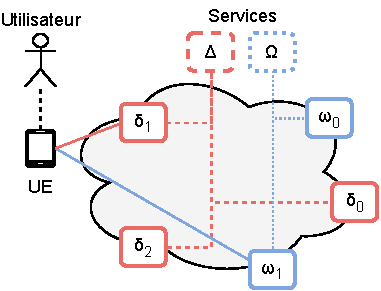
\includegraphics[width=0.4\linewidth]{figs/services-instances.drawio.pdf}
    \caption[Concepts de service et instances]{Le \gl{service/instances}{service} $\Delta$ est déployé sur le réseau en trois \gl{service/instances}{instances} ($\delta_0$, $\delta_1$, et $\delta_2$). Le \gl{service/instances}{service} $\Omega$ est déployé en deux \gl{service/instances}{instances} ($\omega_0$ et $\omega_1$). L’utilisateur obtient le \gl{service/instances}{service} $\Delta$ en utilisant l’\gl{service/instances}{instance} $\delta_1$ et le \gl{service/instances}{service} $\Omega$ en utilisant l’\gl{service/instances}{instance} $\omega_1$.}
    \label{fig:services-instances}
\end{figure}

Cette abstraction permet:
\begin{itemize}
    \item de raisonner sur la distribution spatiale des services sans se limiter aux spécificités du modèle \acren{MEC} de l’\acren{ETSI};
    \item de généraliser les concepts à d’autres paradigmes d’\textit{edge computing} (par ex. le \textit{Fog Computing}~\cite{10.1007/s10115-024-02274-5}) ou de cloud distribué (par ex. \textit{Cloudlet}~\cite{10.1109/ACCESS.2021.3059072}).
\end{itemize} 

\pagebreak
\section{Synthèse}
Nous avons commencé ce chapitre en présentant la 5\textsuperscript{ème} génération de réseaux mobiles et ce qui la distingue des générations précédentes. L’architecture des réseau mobile continue d’évoluer en cherchant toujours à rationaliser davantage les fonctionnalités redondantes et son développement devient « piloté par le logiciel » pour offrir toujours plus de flexibilité aux opérateurs.

Nous avons ensuite présenté le paradigme de l’\textit{edge computing} et l’architecture MEC standardisée par l’ETSI. Dans le chapitre suivant, nous nous intéresserons à l’intégration de ce paradigme avec la 5G.
\end{document}